\section{Recognizable implies regular}\label{app-sec:rec->reg}


\begin{theorem}\label{app-thm:Rec->Reg}
Let $L$ be a language of $\TWT$ graphs. If $L$ is recognizable then it is regular. 
\end{theorem}

\subsection{Pure decomposition of a graph}

We  decompose recursively every pure graph into its \emph{heredidatary pure components}. We relay on the structure analysis of $\TWT$ graphs made in ~\cite{Cosme-LlopezP17}.
On fait cette decomposition en deux étapes.  Every pure graph $G$ can be written as a guarded substitution $G=S[\vec{H}/\vec{x}]$,  where $\vec{H}$ is a list of pure graphs, and  $S$, called the \emph{skeleton} of $G$, is either a word graph,  a multiset graph or a \emph{tree-like} graph, introduced below. \todo{Help from Denis.}

%The graphs $\vec{H}$ are either atomic or pure. The \emph{pure components of $G$} are its first layer components which are pure, together with their pure components.    

\begin{definition}[Tree-like graphs]
A \emph{tree} is a connected acyclic graph (without interface) with no parallel edges\footnote{Acyclicity prevents parallel binary edges, but we want to prevent also parallel unary edges.}.
 
The \emph{rays} of a domain graph $G$ are the binary edges connected to its input, its \emph{spots} are the non-input vertices incident to the rays. 
%We denote by $R(G)$ the labels of the rays. 
 
We say that $G$ is \emph{tree-like} if, when we remove its rays, we obtain a tree whose leaves are spots  (but some spots may not be leaves).   
 
\emph{Left-parallel} graphs are those graphs whose domain is a tree-like graph.
 \end{definition}
 The dashed lines and the red vertices are respectively the rays and the spots of the following domain graphs. 
 The left graph is tree-like, but the right one is not.
  \begin{center}
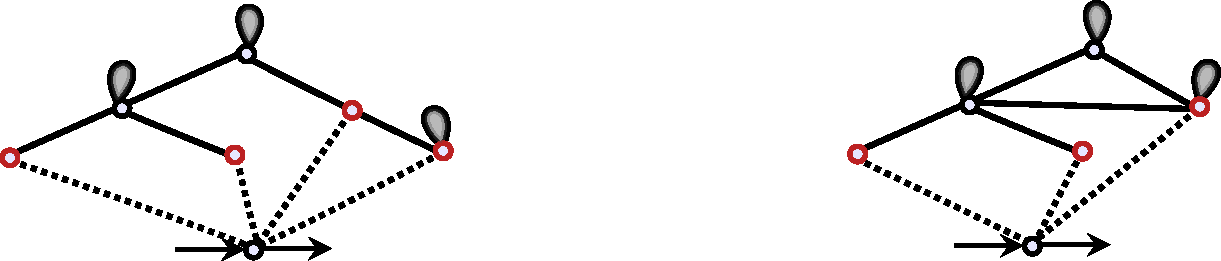
\includegraphics[scale=.4]{tree-like}
\end{center}
%We denote by $\G_\mathsf{s}$, $\G_\mathsf{p}$, $\G_\mathsf{d}$, $\G_\mathsf{t}$, $\G_\mathsf{w}$, $\G_\mathsf{m}$, $\G_\mathsf{\tau}$ and  $\G_\mathsf{u}$ the set of series, parallel, domain, test, word, multiset, tree-like and non-trivial unary graphs.  
%\begin{definition}
%We define \emph{left series-parallel} terms $T_\mathsf{lsp}$, \emph{left parallel} terms $T_\mathsf{lp}$  and \emph{tree-like} terms $T_\tau$ as follows:
%$$\begin{array}{lrlr}
%T_\mathsf{lsp}\qquad\qquad&t, u:=&t\cdot a \cdot b \ \mid\ t \cdot b \ \mid\ t\parallel u \ |\ b&\quad (a\in A_1,\  b\in A_2\cup A_2^\circ).\\
% T_\mathsf{lp}\quad&t:=& u\parallel v&\quad (u,v \in T_\mathsf{lsp}). \\
%T_\tau & t:=&\dom(u\cdot a)& \quad (u\in T_\mathsf{l}).
%\end{array}$$
%We call their graphs respectively \emph{left series-parallel},  \emph{left parallel} and \emph{tree-like} graphs, and denote their set by $\G_\mathsf{lsp}, \G_\mathsf{lp}$ and $\G_{\tau}$ respectively.  
%If $G$ is a tree like graph, we call its \emph{rays} the edges connected to the input. We denote by $R(G)$ the set of letters labeling them.
%\end{definition}
%Tree-like graphs are called so because when we remove their rays, the obtained graph is a tree. Here is an example of a left parallel graph in the left, and a tree-like graph in the right (we did not draw the labels and the orientation of the edges). The rays are the dashed edges. 
%\begin{center}
%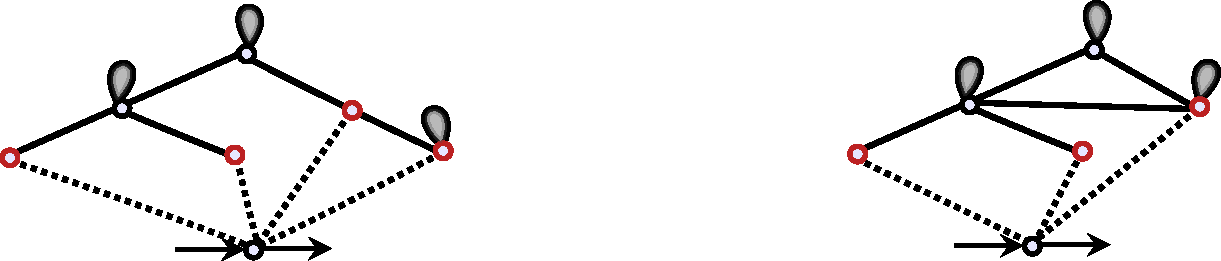
\includegraphics[scale=.4]{tree-like}
%\end{center}
\begin{proposition}[First-layer decomposition]Let $G$ be a pure graph.
\begin{itemize}
\item  If $G$ is parallel, then  $G=M[ \vec{H}/\vec{x}]$, where $M$ is a multiset and the graphs of $\vec{H}$ are series.
\item  If $G$ is a test, then  $G=M[ \vec{H}/\vec{x}]$ where $M$ is a multiset and the graphs of $\vec{H}$ are domain.
\item If $G$ is series, then  $G=W[ \vec{H}/\vec{x}]$ where $W$ is a word and each graph of $\vec{H}$ is either parallel, domain, test or a letter.
\item If $G$ is domain, then  $G=T[ \vec{H}/\vec{x}] $ where $T$ is tree-like, every graph in $\vec{H}$ is either parallel, domain, test or a letter and for every $x\in\vec{x}$, the $x$-labeled edges of $T$ are not rays.
\end{itemize}
The graph $M$, $W$ or $T$ is a \emph{skeleton} of $G$. The graphs of $\vec{H}$ are called the \emph{first-layer components} of $G$, we denote them by $\mathsf{FLC}(G)$. 

The first-layer components of graph are unique, and the skeleton is unique up to renaming and reorientation of its edges.  
\end{proposition}
\begin{proof}
Follows from results in ~\cite{Cosme-LlopezP17}.
\end{proof}
Here is a picture illustrating the first-layer components of a graph:
\begin{center}
Picture
\end{center}
 We define the \emph{hereditary components}  of a graph, recursively, as the union of its first-layer components, with the hereditary components of its first-layer components. 
\begin{definition}[Hereditary decomposition]
 We define the \emph{hereditary components}  of a graph $G$, denoted $\mathsf{HC}(G)$,  recursively as follows:
 $$ \mathsf{HC}(G) = \mathsf{FLC}(G) \cup \underset{H\in\mathsf{FLC}(G)}{\bigcup}  \mathsf{HC}(H)$$
\end{definition}

%\begin{definition}[Pure components of a pure graph] If $G$ is a pure graph, we can write it as:
%$$
%\begin{array}{lll}
%G=W[ \vec{H}/\vec{x}], &W\in \G_\mathsf{w},\ \vec{H}\subseteq \mathcal{G}_\mathsf{p}\cup\mathcal{G}_{\mathsf{u}}, &     \text{if $G$ is series,}\\
%  G=M[\vec{H}/\vec{x}], &M\in \G_\mathsf{m},\  \vec{H}\subseteq \mathcal{G}_\mathsf{s}, & \text{if $G$ is parallel,}\\
%   G=M[\vec{H}/\vec{x}], &M\in \G_\mathsf{m},\  \vec{H}\subseteq\mathcal{G}_{\mathsf{d}},& \text{if $G$ is test,} \\
%   G=T[\vec{H}/\vec{x}, \vec{M}/\vec{y}], & T\in \G_\tau,\  \vec{H}\subseteq \mathcal{G}_\mathsf{p}\cup \G_\mathsf{u},\  \vec{M}\subseteq \mathcal{G}_\mathsf{m}\cap \G_{\mathsf{p}}\ \text{ and }\ \vec{y}\subseteq R(T), &  \text{if $G$ is domain,} 
%\end{array}
%$$
%where all the substitutions above are guarded.  We call the graphs  $W, M$ and $T$ the \emph{skeleton} of $G$, and the graphs $\vec{H}$ and $\vec{M}$ the \emph{first-layer components} of $G$. 
%\end{definition}
 
 
%\noindent Below, the skeleton of a series, parallel and test graph, colored in grey.
%\begin{center}
%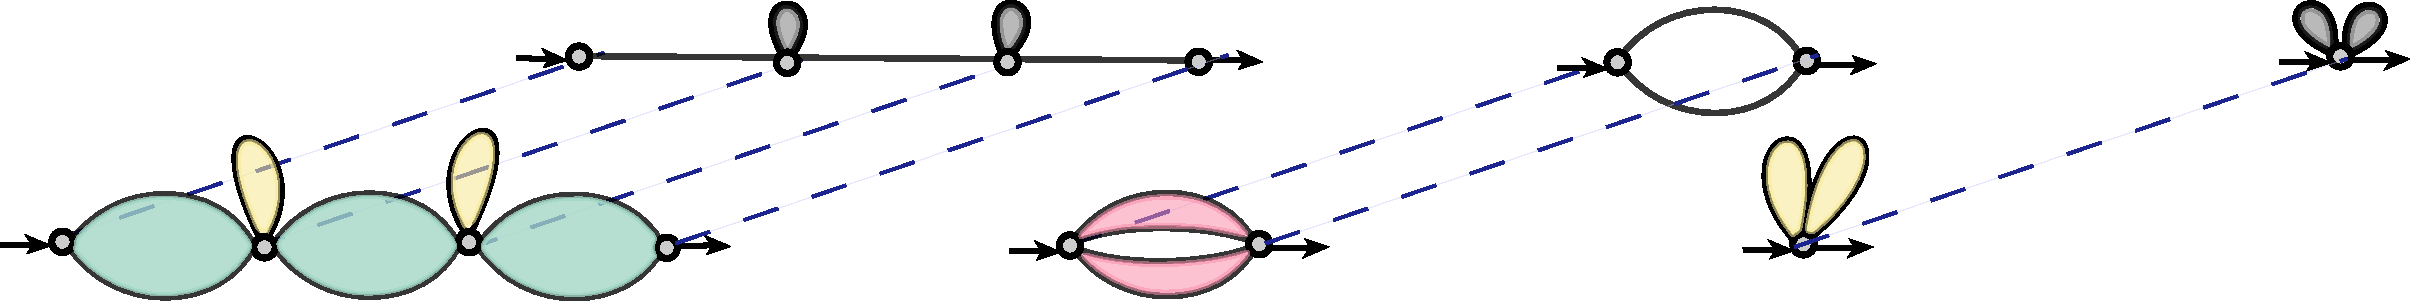
\includegraphics[scale=.35]{skeleton-SPT}
%\end{center}
%The skeleton of a domain graph looks like this.
% \begin{center}
%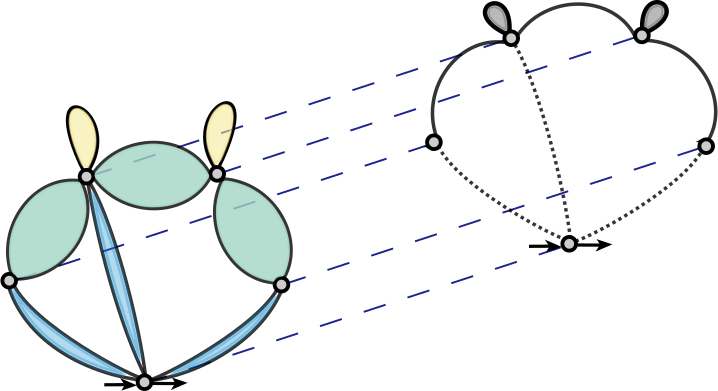
\includegraphics[scale=.35]{skeleton-D}
%\end{center}
%\begin{example} The pure components of the graph $G$ below are  tagged  by the green stars.  At each step of the iteration, we display the skeleton of the graph (linked to the graph by red dashed lines), and the first layer components (linked to the graph by the green dashed lines). 
%\begin{center}
%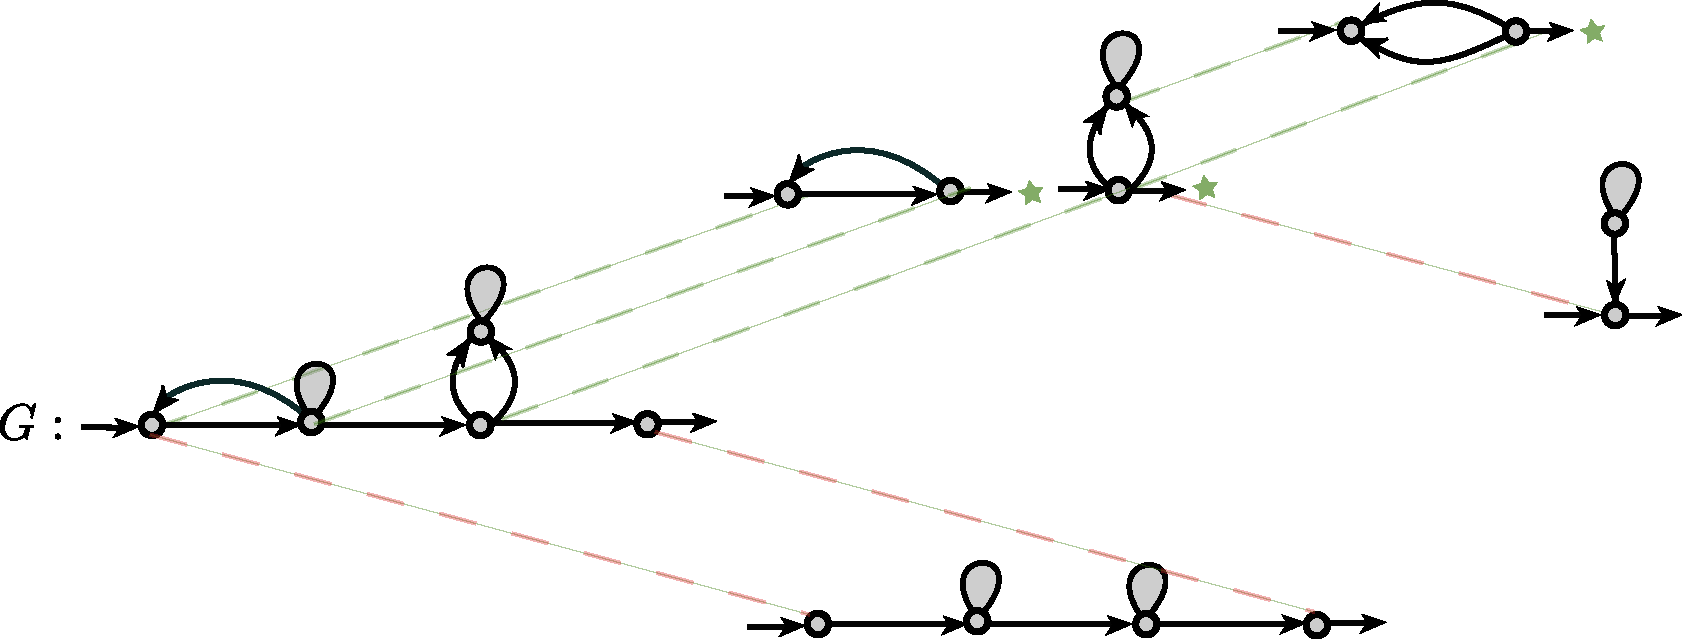
\includegraphics[scale=.4]{skeleton-concrete}
%\end{center}
%\end{example}
\begin{proposition}[Decomposition of impure graphs]
If $G$ is an impure $\TWT$ graph, then $G=M[\vec{H}/\vec{x}]$ where $M$ is a multiset, $\vec{H}$ are pure graphs and this substitution is guarded. 

 The \emph{first-layer components} of $G$ are the graphs $\vec{H}$ appearing in any such decomposition, which is not unique in general. 
\end{proposition}
\begin{remark} Notez qu'on n'a \textbf{pas} défini une decomposition herediataire dans le cas impure. \todo{french}
\end{remark}
Un premier resultat dont on aura besoin, c'est que lorqu'on remplace un hereditary component d'un graph par une letter, alors cette lettre est guardée.

\begin{proposition}
If $G$ is a pure graph and $M$ a hereditary component of $G$ of type  $\tau$, then $x$ is $\tau$-guarded in $G[x/M]$.

If $G$ is an impure $\TWT$ graph and $M$ a first-layer component of $G$ of type $\tau$, then $x$ is $\tau$-guarded in $G[x/M]$.


\end{proposition}

En plus d'être guardée, elle occuppe une position principale. Technical definition.\todo{en dire plus?}

\begin{definition}[principal letter]
We say that a letter $x$ is \emph{secondary} in a graph $G$ if there is a unary module $M$ of the form $\dom(x)$ or $\dom(x\parallel H)$ where $H$  is a module of $G$.
A letter is \emph{principal} if it is not secondary.
\end{definition}
Here is a picture illustrating the two cases where  $x$ is secondary:
% 
%\begin{lemma}\label{app-lem:no-pure-comp}
%Let $G$ be a graph such that $\mathsf{pure}(G)=\emptyset$.
%If $G$ is series, then it is a word graph. If $G$ is parallel, test or impure, then it is a multiset graph. If $G$ is domain, then it is a tree-like graph. 
%\end{lemma}


\begin{lemma}\label{app-lem:pure-substitution}
Let $G, H$ be pure graphs such that $G[H/x]$ is guarded and suppose that $x$ is principal in $G$. We have: 
$$\mathsf{HD}(G[H/x])\subseteq  \mathsf{HD}(G)[H/x] \cup \mathsf{HD}(H) \cup \set{H} $$
\end{lemma}
\begin{proof}
We proceed by induction on the structure of $G$. 
\end{proof}


\subsection{Type respecting algebra}

\begin{definition}
Let  $\A$ be an algebra whose domain is $D$. We say that $\A$ is \emph{type respecting} if we can find subsets $D_\mathsf{atomic}$, $D_\mathsf{pure}, D_\mathsf{impure}, D_\mathsf{s}, D_\mathsf{p}, D_\mathsf{d}, D_\mathsf{t}$, $D_\mathsf{lp}$ and $D_\mathsf{\tau}$ of the domain $D$, such that for every term $t$, its graph is pure, impure,  series, parallel, domain, test, left-parallel or tree-like, if and only if the evaluation of $t$ belongs to theses sets respectively.  
\end{definition}

\begin{lemma}\label{app-prop:type-respecting-rec}
If $L$ is a recognizable language of $\TWT$ graphs, then  it is recognizable by a type respecting algebra.
\end{lemma}

\begin{proof}\todo{french}
D'abord remarquer que les tree like graphes sont generés par une syntaxe. Et c'est ça qui fait que c'est facile de se rappeler d'eux.
We need to remember only a finite amount of information to know whether a graph is in each of these sets. 
\end{proof}





\subsection{Recognizable implies regular}

We can proceed to the Proof of Theorem~\ref{app-thm:Rec->Reg} Let $L$ be a recognizable language. By Prop.~\ref{app-prop:type-respecting-rec}, we can assume that $L$ is recognized by a type respecting algebra, and keep the same notations used there. Let $h$ be a homomorphism recognizing $L$, and $F\subseteq D$ such that $L=h^{-1}(F)$. We define $L_r$ as the language of graphs whose image (by $h$) is $r$. Our goal is to show that $L_r$ is regular for every $r\in D$. This is enough to conclude because 
$L=\underset{r\in F}{\bigcup}L_r$.
\medskip

First, we will show that $L_r$ is regular when {$r\in D_\mathsf{pure}$}. 
\medskip

  Let $A_\mathsf{pure}$ be a alphabet containing a binary letter for each element of the set $D_\mathsf{s}\cup D_\mathsf{p}$, and a unary letter for each element of  $D_\mathsf{d}\cup D_\mathsf{t}$. If $r\in D_{\mathsf{pure}}$, we denote by $x_r$ its corresponding letter in $A_\mathsf{pure}$. We extend $h$  to terms over  $A\cup A_\mathsf{pure}$, by letting $h(x_r)=r$ for every $r\in D_\mathsf{pure}$.
\smallskip

Let $P \subseteq  D_{\mathsf{pure}}$, $\Sigma\subseteq A_\mathsf{pure}$ and $r\in D$. We define $L^{P,\Sigma}_r$ as the set of graph terms over the alphabet $A\cup \Sigma$ defined as follows. We let $G\in L^{P,\Sigma}_r$  if and only if:
\begin{enumerate}
\item The image of $G$ is $r$.
\item The image of every pure components of $G$ belongs to $P$.
\item For every $v\in D_\mathsf{\tau}$ such that $x_v$ appears in $G$, $x_v$ is principal and $\tau$-guarded in $G$.
\end{enumerate}


\noindent We show, by induction on the size of $P$, that $L^{P, \Sigma}_s$ is regular  if  the letters associated to $P$ and the set $\Sigma$ are disjoint. We start by the inductive step.
\smallskip

 \noindent \textbf{Inductive step.} Suppose that $P=Q\uplus \set{v}$. We prove the following equality:
$$L^{P,\Sigma}_r=L^{Q,\Sigma\cup\set{x_v}}_r[\mu x_v. L^{Q,\Sigma\cup\set{x_v}}_v/x_v][L^{Q,\Sigma}_v/x_v] \qquad\qquad(\star) $$
Substitutions and iterations in $(\star)$ are guarded thanks to the conditions 3 and 4 above. 
Using this equality and the induction hypothesis, we can conclude that the language $L^{P,\Sigma}_r$ is regular. 


The right-to-left implication follows from Lem.~\ref{app-lem:pure-substitution}.  Let us show the other inclusion. 

\noindent A \emph{$v$-component} of a graph is a pure component of this graph whose image by $h$ is $v$.  The \emph{$v$-reduct} of a graph is the graph obtained by replacing every $v$-component by the letter $x_v$, such that the resulting graph has no $v$-components.  Let $G$ be a graph in  $L^{P,\Sigma}_r$,  we let: 
\begin{itemize}
\item $H$ be the $v$-reduct of $G$,
\item $S$ be the set of $v$-reducts of the $v$-components of $G$.
\item $T$ be the set of $v$-components of $G$, which do not contain further $v$-components.
\end{itemize}
We have the following inclusions: 
$$G\in H[\mu x_r. T/x_r][S/x_r],\quad H\subseteq L^{Q,\Sigma\cup\set{x_v}}_r,\quad S\subseteq L^{Q,\Sigma\cup\set{x_v}}_v\ \  \text{ and }\ \ T\subseteq L^{Q,\Sigma}_v.$$
This concludes the left-to-right inclusion of $(\star)$, and  the inductive step. Now let us treat the base case.  We have two base cases, one of them will make a call to the inductive step. 
\medskip


 \noindent \textbf{Base case 1.} $P$ is empty and $r\in D_\mathsf{s}\cup D_\mathsf{p}\cup D_\mathsf{t}$. Then the graphs of $L^{\emptyset,\Sigma}_r$ are either word graphs or multiset graphs. Their regularity follow from the case of words and commutative words.
\medskip

\begin{observation}
Using base case 1 and the inductive step, we have that 
$L^{P,\Sigma}_r$ is regular if $r\in D_\mathsf{s}\cup D_\mathsf{p}\cup D_\mathsf{t}$ and $P\subseteq D_\mathsf{s}\cup D_\mathsf{p}\cup D_\mathsf{t}$. 
\end{observation}
\medskip

\noindent \textbf{Base case 2.} $P$ is empty and $r\in D_\mathsf{d}$.  The graphs of $L^{\emptyset,\Sigma}_r$ are tree-like graphs. 
Let $S$ be the set of pairs $(v,a)$ such that $v\in D_{\mathsf{lp}}$, $a\in A_1$ and $r=\dom(v\cdot a)$. We have that:
$$ L^{\emptyset, \Sigma}_r=\underset{(v,a)\in S}{\bigcup}\dom\big({L^{D_\mathsf{s}\cup D_\mathsf{t},\Sigma}_v\cdot a}\big)$$
because left parallel graphs do not have unary pure components. The set $ L^{\emptyset, \Sigma}_r$ is regular thanks to the observation above. 
\medskip

When $r\in D_\mathsf{atomic}$,  $L_r$ is regular because it is finite. 
\medskip

Let us show that $L_r$ is regular when $r\in D_\mathsf{impure}$.
Note that
$$L_r= L^{\emptyset, A_\mathsf{pure}}_r[L_v/x_v, v\in D_\mathsf{pure}]$$
The language $L^{\emptyset, A_\mathsf{pure}}_r$ is a language of multiset graphs, it regularity follows from the case of commutative words. The languages $L_v$ are regular because $v$ is pure, and this case was treated above. This concludes the proof. 